%%%%%%%%%%%%%%%%%%%%%%%%%%%%%%%%%%%%%%%%%
% Stylish Article
% LaTeX Template
% Version 2.1 (1/10/15)
%
% This template has been downloaded from:
% http://www.LaTeXTemplates.com
%
% Original author:
% Mathias Legrand (legrand.mathias@gmail.com)
% With extensive modifications by:
% Vel (vel@latextemplates.com)
%
% License:
% CC BY-NC-SA 3.0 (http://creativecommons.org/licenses/by-nc-sa/3.0/)
%
%%%%%%%%%%%%%%%%%%%%%%%%%%%%%%%%%%%%%%%%%

%----------------------------------------------------------------------------------------
%	PACKAGES AND OTHER DOCUMENT CONFIGURATIONS
%----------------------------------------------------------------------------------------

\documentclass[fleqn,10pt]{SelfArx} % Document font size and equations flushed left

\usepackage[english]{babel} % Specify a different language here - english by default

\usepackage{lipsum} % Required to insert dummy text. To be removed otherwise
\usepackage{graphicx}
%----------------------------------------------------------------------------------------
%	COLUMNS
%----------------------------------------------------------------------------------------

\setlength{\columnsep}{0.55cm} % Distance between the two columns of text
\setlength{\fboxrule}{0.75pt} % Width of the border around the abstract

%----------------------------------------------------------------------------------------
%	COLORS
%----------------------------------------------------------------------------------------

\definecolor{color1}{RGB}{0,0,90} % Color of the article title and sections
\definecolor{color2}{RGB}{0,20,20} % Color of the boxes behind the abstract and headings

%----------------------------------------------------------------------------------------
%	HYPERLINKS
%----------------------------------------------------------------------------------------

\usepackage{hyperref} % Required for hyperlinks
\hypersetup{hidelinks,colorlinks,breaklinks=true,urlcolor=color2,citecolor=color1,linkcolor=color1,bookmarksopen=false,pdftitle={Title},pdfauthor={Author}}

%----------------------------------------------------------------------------------------
%	ARTICLE INFORMATION
%----------------------------------------------------------------------------------------

\JournalInfo{National University of Singapore, ISS, 26-Oct, 2015} % Journal information
\Archive{Computational Intelligence II} % Additional notes (e.g. copyright, DOI, review/research article)

\PaperTitle{An Exploration of Implementing GA in Fractals} % Article title

\Authors{Pan An\textsuperscript{1}(A0134556A), Devendra Desale\textsuperscript{1}(A0134465E)} % Authors
%\affiliation{\textsuperscript{1}\textit{Department of Biology, University of Examples, London, United Kingdom}} % Author affiliation
%\affiliation{\textsuperscript{2}\textit{Department of Chemistry, University of Examples, London, United Kingdom}} % Author affiliation
%\affiliation{*\textbf{Corresponding author}: john@smith.com} % Corresponding author

\Keywords{Genetic Algorithm, Fractals, JuliaSet} % Keywords - if you don't want any simply remove all the text between the curly brackets
\newcommand{\keywordname}{Keywords} % Defines the keywords heading name

%----------------------------------------------------------------------------------------
%	ABSTRACT dalianligongdaxue ruanjainxuyean
%----------------------------------------------------------------------------------------

%\Abstract{\lipsum[1]~}
\Abstract{
 Genetic algorithm(GA) is a search heuristic that mimics the process of natural selection.
 Genetic algorithm can help search and optimize while at the same time, remain a small amount of randomness to the original problems.
 This paper presents some exploration of combining fractals with genetic algorithms. Different types of fractals have been discussed together with multiple ways of implementation of GA. We specifically surveyed and modeled on MaldelbrotSet and JuliaSet how genetic algorithms can be used to enhance the process. The presented model covers both esthetical and speed optimization level. Though genetic algorithm is not able to provide optimization for real time generation of fractals, the randomness of the algorithm does help provide more vivid visual effect to the graphics.
 %%%%%%%%%%%%%%% make some changes and add detailed about what you did
}
%----------------------------------------------------------------------------------------

% 41.3529999256134 seconds for 3200*2400

\begin{document}

\flushbottom % Makes all text pages the same height

\maketitle % Print the title and abstract box

\tableofcontents % Print the contents section

\thispagestyle{empty} % Removes page numbering from the first page

%----------------------------------------------------------------------------------------
%	ARTICLE CONTENTS
%----------------------------------------------------------------------------------------

\section*{Introduction} % The \section*{} command stops section numbering

\addcontentsline{toc}{section}{Introduction} % Adds this section to the table of contents

A fractal is a natural phenomenon or a mathematical set that exhibits
a repeating pattern that displays at every scale. It is also known as
expanding symmetry or evolving symmetry. If the replication is exactly
the same at every scale.

% add bibs to this part to make it look cool and fun
"As far as the laws of mathematics refer to reality, they are not certain, and as far as they are certain, they do not refer to reality." Quoting from Albert Einstein, an intuitive understanding about chaos. Recognizing the chaotic, fractal nature of our world can give us new insight, power, and wisdom. For example, by understanding the complex, chaotic dynamics of the atmosphere, a balloon pilot can "steer" a balloon to a desired location. By understanding that our ecosystems, our social systems, and our economic systems are interconnected, we can hope to avoid actions which may end up being detrimental to our long-term well-being.

Mandelbrotset, Juliaset, strange attractors are some of the most famous fractal models that have been known by people for decades. Fractals models can be either exact or combined with chaos. Previous work of combining genetic algorithms has been conducted on some classic fractal models. Ashlock et. al.~\cite{ashlock2006evolutionary} presented  a collection of fitness functions that permit three-parameter evolutionary search of the Mandelbrot set to locate interesting views. The collection includes several pieces of graphics that is generated with GA. J. McCormack \cite{mccormack2005open}  researched and listed five 'open problems'  of  evolutionary music
and art.
Another example of using algorithmic ways to generate more vivid art

is deep dream~\cite{deep_dreams}.
Each problem is explained and the impetus and background for it is described
in the context of creative evolutionary systems.




Despite the colors, the shape and the complexity, these fractals have simple models at the back. In this paper we descriped a way we found to implement genetic
algorithm into fractal arts by using the Mandeltweak as one of the key
factors for genetic optimization.
 In order to achieve something from this experimental exploration, the following principles are taken into consideration when building the model:

\begin{itemize}
\item Unpredictability
\item Order / Disorder Chaos is not simply disorder
\item Mixing(Different patterns, or generating new patterns)
\end{itemize}

The paper is organized as the following description: in Chaper. 1 several fractal models are presented together with some tests in the visual effects. Chapter. 2 contains some of the principles and ideas we had when designing.
 Chapter. 3  contains our models and some details for combining genetic algorithms into fractals.


%% put all these to other places
\href{http://giphy.com/gifs/l41lUTY3yTLywvYRO?utm_source=facebook&utm_medium=embed&utm_campaign=share}{\bf This is the link to the Juliaset animation.}
%%%%    http://i.giphy.com/3oEduP6LzD2FmfkwMg.gif
%------------------------------------------------

\section{Classic Fractals}
The word "fractal" often has different connotations for laypeople than for mathematicians, where the layperson is more likely to be familiar with fractal art than a mathematical conception. The mathematical concept is difficult to define formally even for mathematicians, but key features can be understood with very simple mathematics.

\subsection{MandelbrotSet}
MandelbrotSet was one of the most famous and classical fractals. The
Mandelbrot set is the set of complex numbers 'c' for which the
sequence {$c, c^2+c, (c^2+c)^2+c, ((c^2+c)^2+c)^2+c, ...$} does not
approach infinity. It is named after the mathematician Benoit
Mandelbrot, who studied and popularized it. Mandelbrot set images are
made by sampling complex numbers and determining for each whether the
result tends towards infinity when a particular mathematical operation
is iterated on it.


More precisely, the Mandelbrot set is the set of values of c in the
complex plane for which the orbit of 0 under iteration of the complex
quadratic polynomial
$$Z_{n+1} = Z^2_n + c$$
remains bounded.



\begin{figure}[h!]
  \centering
      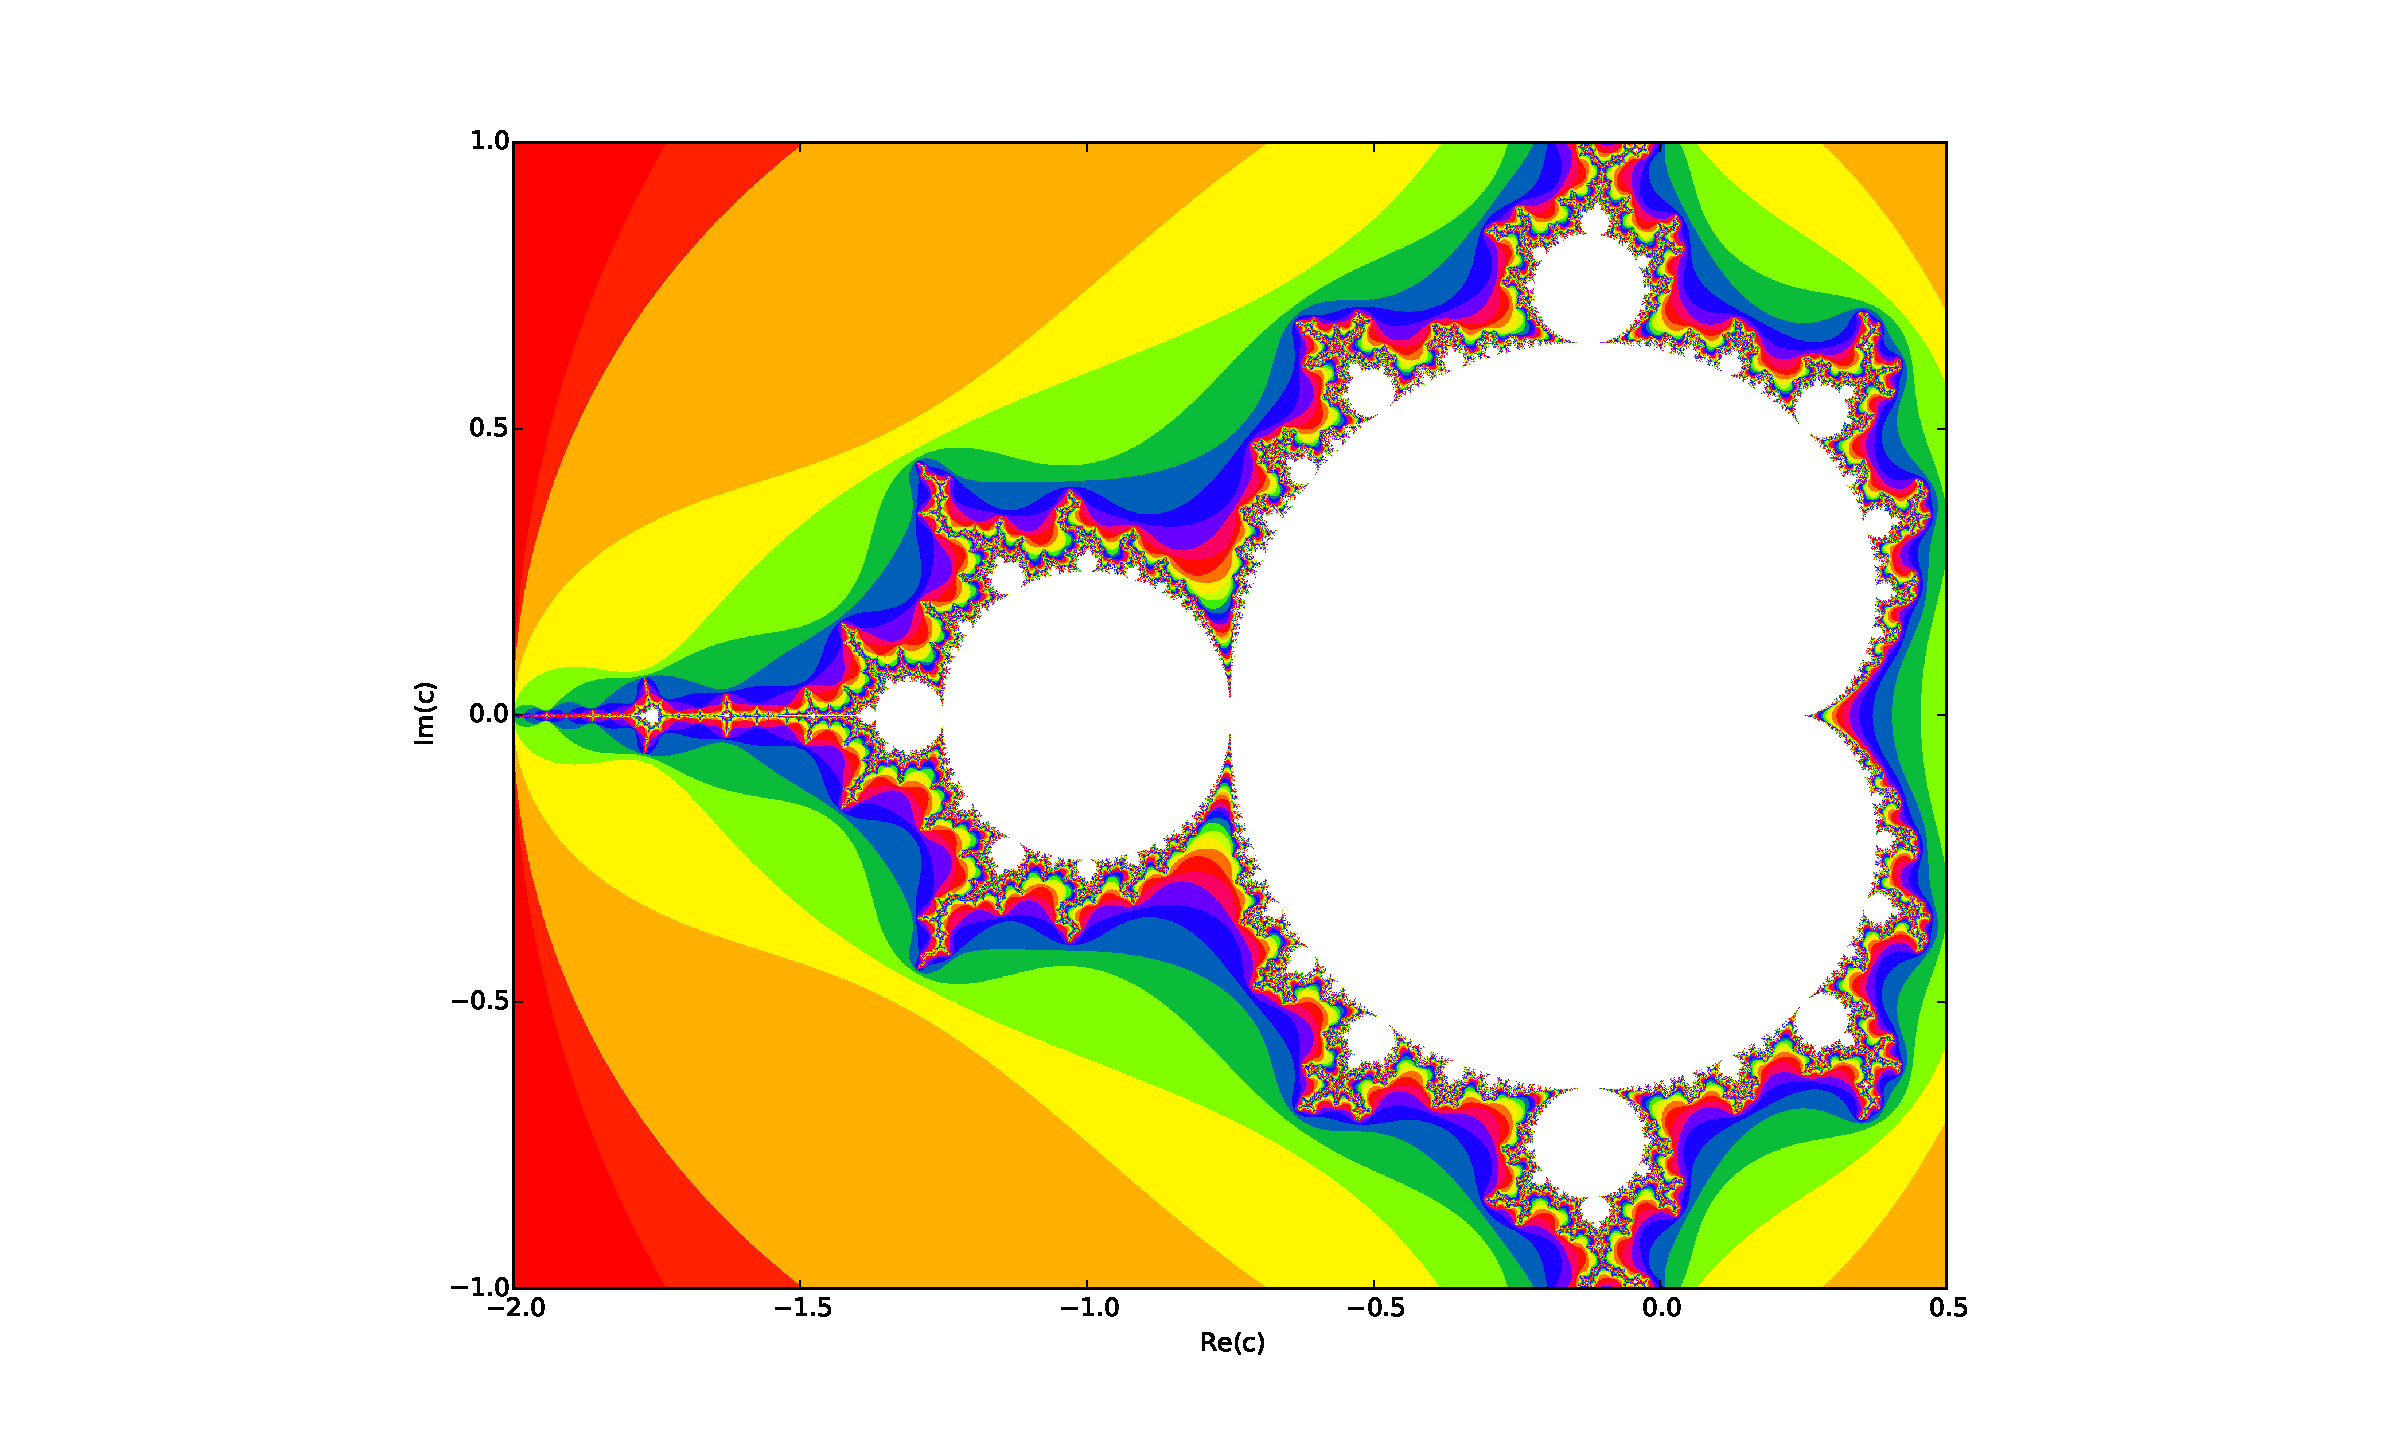
\includegraphics[width=0.5\textwidth]{figure_1.pdf}
  \caption{MandelbrotSet Generated with Python}
\end{figure}


\subsection{JuliaSet}

In the context of complex dynamics, a topic of mathematics, the Julia
set and the Fatou set are two complementary sets  defined from a
function. JuliaSet has a close connection to MandelbrotSet. Formal
definition and description can be found on Wikipedia~\cite{julia_wiki}.


Unlike MandelbrotSet, Julia Set itself has a lot of forms. Julia Set
represents  a set of fractals that satisfies specific mathematical
bonds.

\begin{figure}[h!]
  \centering
      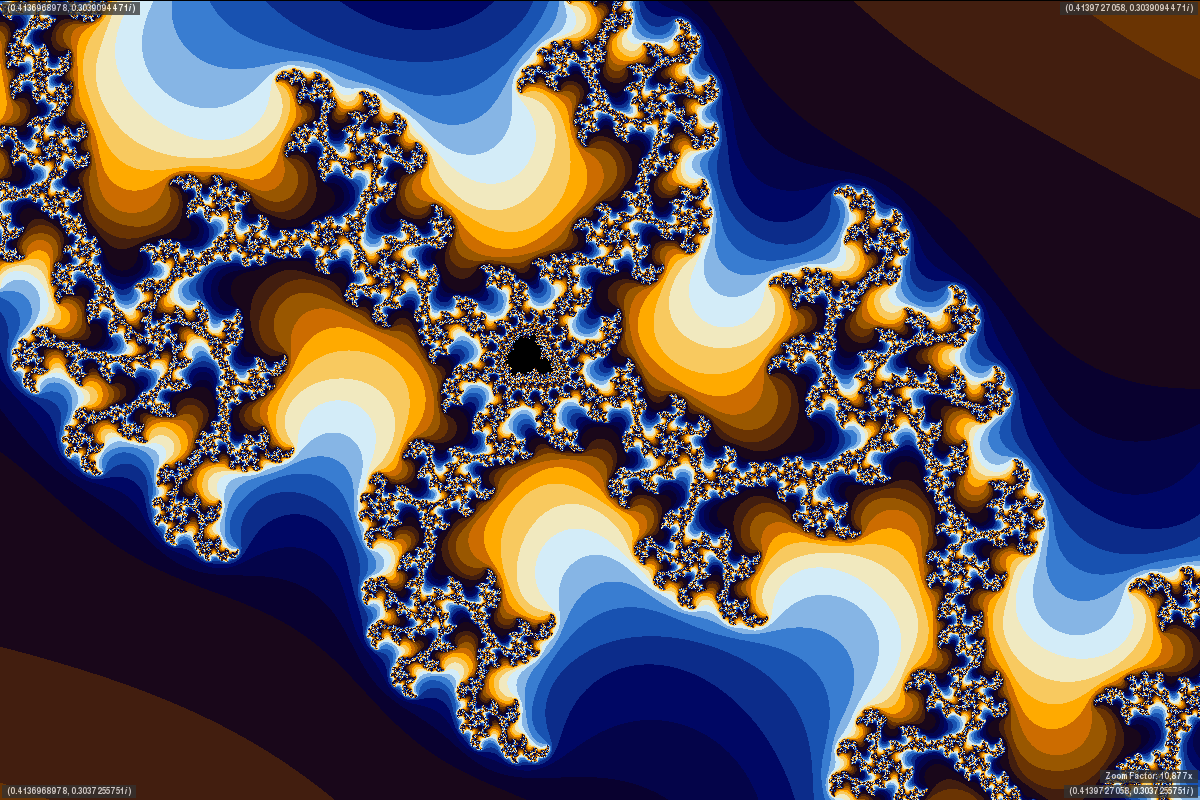
\includegraphics[width=0.4\textwidth]{698.png}
  \caption{An Example of Julia Set}
\end{figure}


Figure. 2 shows an example of Julia Set we generated with simple
python script. We also generated an animation about Julia
Set. \href{http://giphy.com/gifs/l41lUTY3yTLywvYRO?utm_source=facebook&utm_medium=embed&utm_campaign=share}{\bf
  This is the link to the Juliaset animation.}

In a word: you can calculate a Julia set from any point within a
certain limit (if you take large values the result might be empty,
though). If your chosen point is not part of the Mandelbrot set (it is
not a black pixel when visualized), the resulting Julia set will
contain islands. However if you choose a point that is part of the
Mandelbrot set (it is a black pixel when visualized) the resulting
Julia set will be contiguous.

Also Figure. 3 shows
the connection between MandelbrotSet and Julia Set:



\begin{figure}[h!]
  \centering
      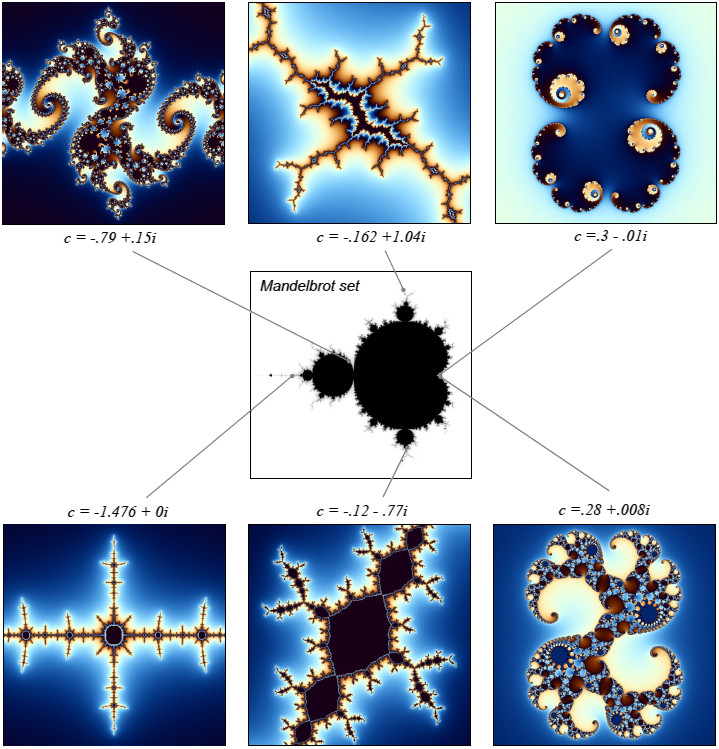
\includegraphics[width=0.4\textwidth]{julia_mandel.jpg}
  \caption{Connection Between JuliaSet and MandelbrotSet}
\end{figure}


\subsection{Fractal Flame}
Fractal flames are a member of the iterated function system class of
fractals created by Scott Draves in 1992. Draves' open-source code was
later ported into Adobe After Effects graphics software and translated
into the Apophysis fractal flame editor.~\cite{fractal_flames}
Fractal flames differ from ordinary iterated function systems in some
ways.

Following picture shows an example of fractal flame:

\begin{figure}[h!]
  \centering
      
\includegraphics[width=0.3\textwidth]{fractal_flame.jpg}
  \caption{Fractal Flame}
\end{figure}


\section{Principles}


The Mandelbrot equation was discussed in the second chapter, where z
and c are complex numbers and c is a location in the complex plane
being tested. The function is applied many times, with the output
value of z from each iteration being used as input for the next
iteration. During iteration, if the value of z exceeds a magnitude of
2, then iteration halts and we declare that location in c as outside
of the Mandelbrot Set (white). Otherwise, c lies inside of the Set
(black).

If the function were iterated only once at each $c$, the result would be a round shape, analogous to a single cell before subdividing into a multicelullar organism. Each time the function is iterated, the approximation of the Set becomes more refined, and the boundary reveals more bays and peninsulas.
Fractal self-similarity increases.

If instead of squaring the value of z, you cube it $(z_{n+1} = z_n^3 +
c)$, the result would be totally different. The following figure shows
an example of MandelbrotSet with equation$(z_{n+1} = z_n^4 +
c)$.



\begin{figure}[h!]
  \centering
      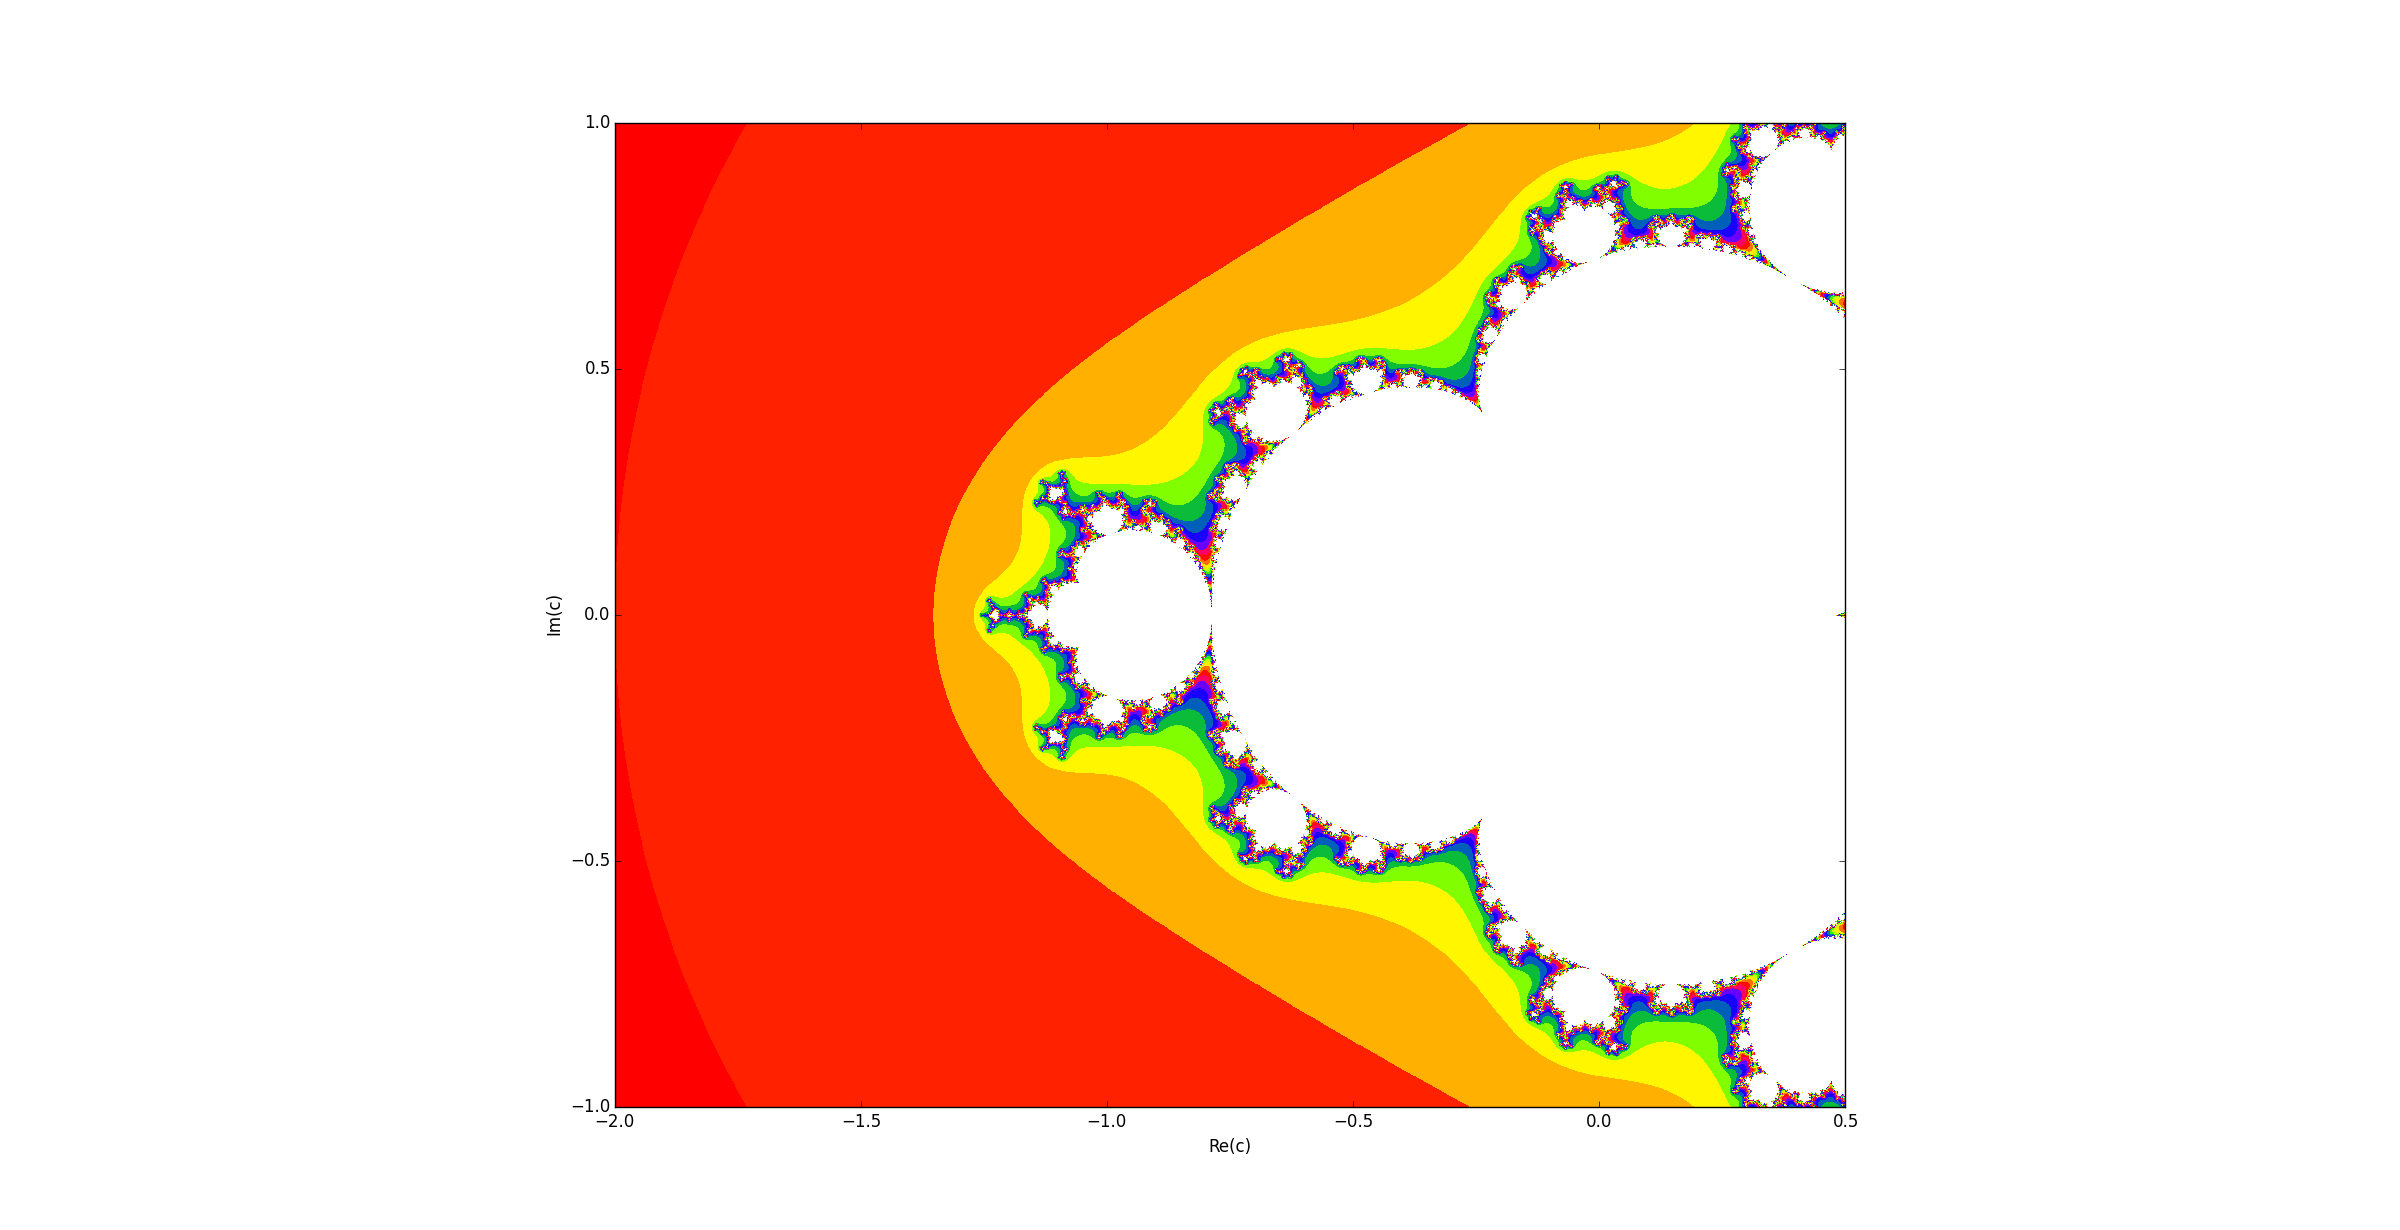
\includegraphics[width=0.6\textwidth]{figure_2.png}
  \caption{Another MandelbrotSet}
\end{figure}

With different equations and settings we can configure and generate
dramatic amount of settings we can create a large genetic space. In
next chapter we will give the specificity of the algorithm and idea.


\section{Using Genetic Algorithm}

Any time you have a set of computer-generated images whose variety can be encoded as a large set of parameters, you have a good candidate for using a genetic algorithm to search the large space of possible images. So I used a variation on the genetic algorithm to interactively search for cool artworks.


\subsection{Genetic Space and Optimization Target}
In this paper we used a random image as a fitness metric, to find out
if the Mandelbrot Set could be coerced into taking on the appearance
of my face? So I developed a way to compare a 50x50-pixel Mandeltweak
to a 50x50-pixel image of my face. I then generated a population of
Mandeltweaks, each based on a unique genome. A genetic algorithm was
used to find Mandeltweaks that most closely-approach the likeness of
my face.

The fact that the Mandeltweaks were not able to accurately approach
our likeness, and the fact that they have their own genetic signature,
which is not at all human - this made for some strange images -
looking like a human head at first glance, but upon closer inspection,
showing a non-human genetic signature.

\subsection{Convergence}

The scheme is as follows: A population of genomes is created, which
starts out completely random. Then, random genomes are chosen from the
pool to mate and create an offspring, using crossover. The offspring
genotype is used to generate a new Mandeltweak, which is compared to
the ideal image and given a fitness value. The new offspring replaces
the least-fit individual in the population. This process is repeated
many times. Over time, the average fitness increases, as well as the
similarity to the ideal image.


Mandeltweaks have particular attributes that make them unable to
evolve to emulate all possible images - although they can approximate
certain images to some degree.


\subsection{Tests and Discussion}

We  ran MandelbrotSet tweak with some tools and a random
image. The following figure shows the result of the testing:


\begin{figure}[h!]
  \centering
      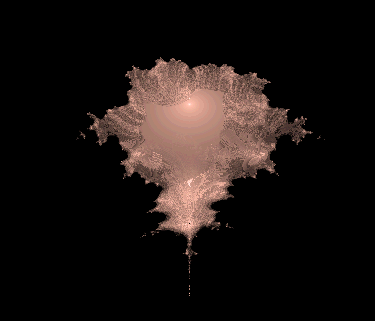
\includegraphics[width=0.4\textwidth]{tweak.png}
  \caption{MandelbrotSet with GA}
\end{figure}

\begin{figure}[h!]
  \centering
      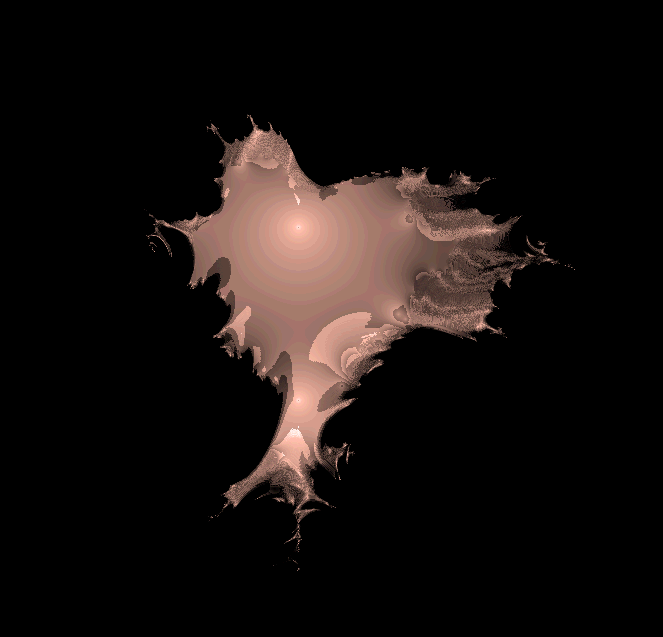
\includegraphics[width=0.4\textwidth]{tweak2.png}
  \caption{Another Example of Tweak Optimization}
\end{figure}


The esthetical result might be appealing to normal people, but we
believe that with proper optimization in the tool we can achieve a
better result. A better version was provided by the original author of
the idea:


\begin{figure}[h!]
  \centering
      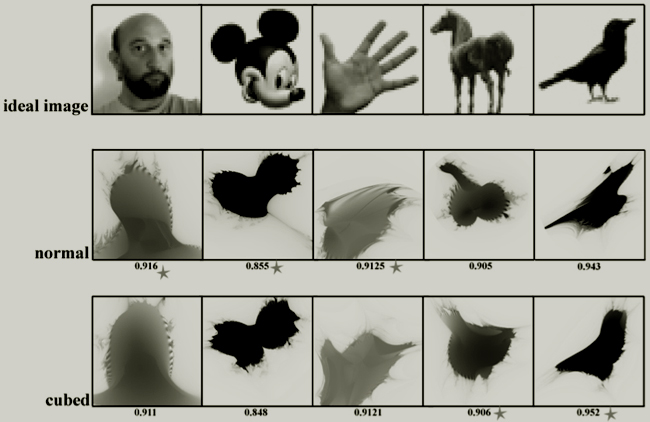
\includegraphics[width=0.4\textwidth]{test.jpg}
  \caption{Test of GA MandelbrotSet}
\end{figure}

The author  included a special tweak based on "Mandelbrot cubed" (which includes many more genes) to see if its larger phenotype space would have any more imitative abilities.
Yet many of the distinctive aspects of the image were not picked up, such as eyes, legs, and fingers. And it wasn't able to imitate Mickey Mouse's face, which might be good, since I don't want to get sued by Disney.


\section*{Conclusion} % The \section*{} command stops section numbering
Geneticl algorithm can be implemented the real world problems. Using
genetic algorithm(along with other machine learning techniques) in
visual arts can help people generate more innovated ideas. With some
proper control in the system we could achieve a very good result in
the art world.

%----------------------------------------------------------------------------------------
%	REFERENCE LIST
%----------------------------------------------------------------------------------------
\phantomsection
\bibliographystyle{unsrt}
\bibliography{sample}

%----------------------------------------------------------------------------------------

\end{document}

%%% Local Variables:
%%% mode: latex
%%% TeX-master: t
%%% End:
